\begin{tikzpicture}
\draw [](-2.92,2.32) node (v1) {} .. controls (-3.26,2.06) and (-3.26,0.54) .. (-2.92,0.32) node (v2) {};

\draw [draw=black,fill=black!20](-0.68,2.32) node (v1) {} .. controls (-1.08,2.06) and (-1.08,0.54) .. (-0.68,0.32) node (v2) {};
\draw [white, fill=black!20](-0.68,2.32) -- (1.56,2.32) -- (1.56,0.32) -- (-0.68,0.32);


\draw [draw=black,fill=black!60](-0.93,1.78) node (v1) {} .. controls (-0.99,1.59) and (-0.99,1.14) .. (-0.95,0.94) node (v2) {};
\draw [draw=black,fill=black!60](-0.93,1.78) -- (0.72,1.78) -- (0.72,0.94) -- (-0.95,0.94);


\draw [draw=black,fill=white] (0.48,1.36) node (v3) {3} ellipse (0.2 and 0.3);
\draw [draw=black,fill=black](0.28,1.66) -- (0.28,1.06);

\draw [draw=black,fill=white] (-3.4,1.36) node (v3) {1} ellipse (0.2 and 0.3);
\draw [draw=black,fill=black](-3.6,1.7) -- (-3.6,1.06);


\draw [draw=black,fill=black] (-2.9,1.7) rectangle (-3,1);
\draw (-2.9,1.3) -- (-2.6,1.7) -- (-2.6,1) -- (-2.9,1.3);
\node at (-2.7,1.34) {\small{2}};
\node at (-1.7,1.54) {\small{c[n]}};

\draw[->,dashed] (-2.6,1.36) node[right=0.5,above]{\small{}}-- (0.28,1.36);



\draw [->](-1.14,-1.76) -- (-1.14,-0.2) -- (-2.94,-0.2) -- (-2.94,1);
\node at (0,2) {\small{Ear Canal}};
\node[anchor=south west,inner sep=0] at (1.9,0.3) {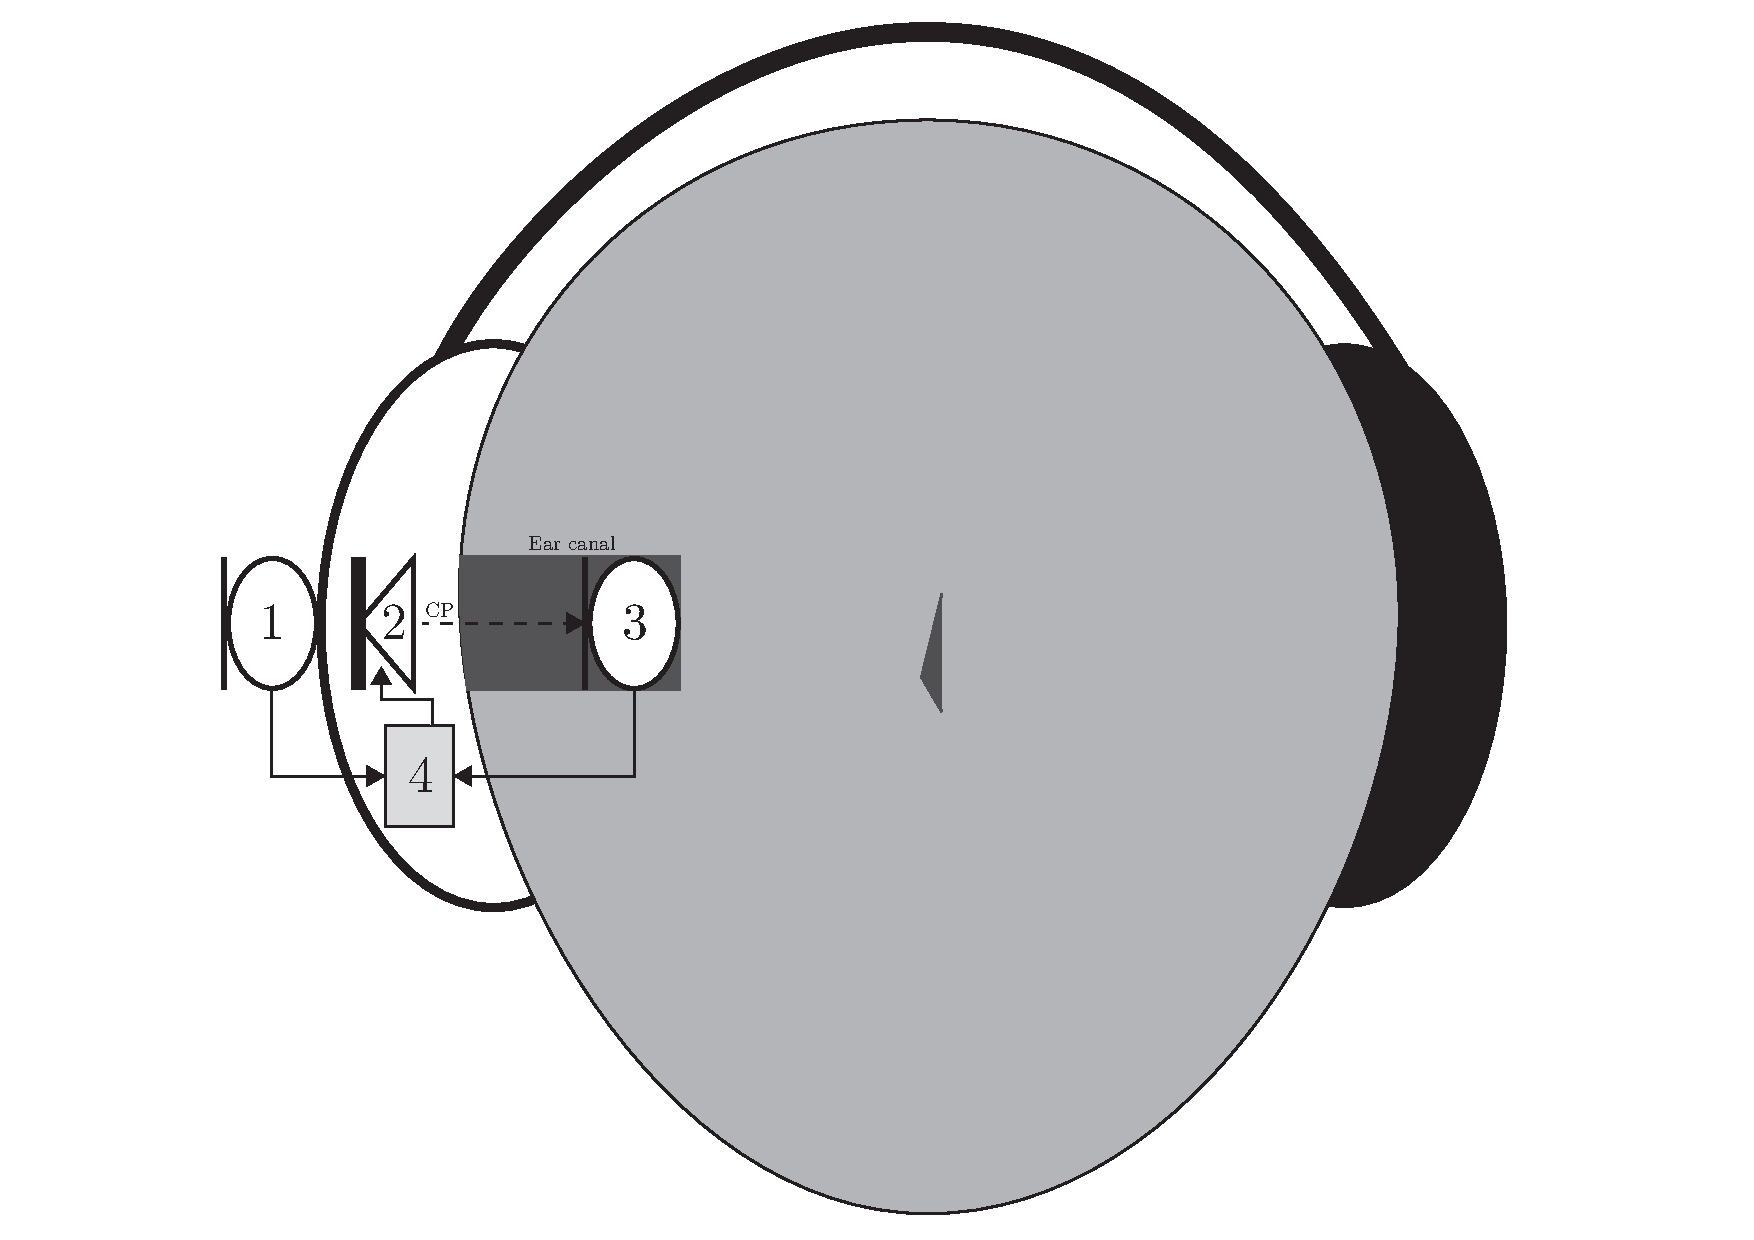
\includegraphics[width=3cm]{figures/BasicOverview}};

\draw  (3.14,1.65) rectangle (2.14,0.95);

\draw (1.56,1.31) -- (2.14,1.31);
\draw  (1.56,2.32) rectangle (-3.7,0.32);
\draw  (-5,-1.75) rectangle node[text width=2cm,align=center] {ADC \& Antialiasing filter} (-2.86,-3.25);
\draw  (-5,-6) rectangle node[text width=2.5cm,align=center] {Cancellation \\ path}(-2.75,-7.5);
\draw  (-1.23,-6) rectangle node[text width=2.5cm,align=center] {Adaptive FXLMS Algorithm} (1.27,-7.5);

\draw  (-3.45,-3.79) rectangle node[text width=1.5cm,align=center,fill=white] {Control filter} (-1.58,-5.29);
\draw  (-2.08,-1.75) rectangle node[text width=2.5cm,align=center] {DAC \& \\ Reconstruction filter}(0.37,-3.25);
\draw  (0.77,-1.75) rectangle node[text width=2cm,align=center] {ADC \& Antialiasing filter}(2.91,-3.25);

\draw  (-5.71,-0.69) rectangle (3.55,-7.76);
\node at (-5.06,-0.99) {DSP(4)};
\node [text width=2cm,align=center] at (-3.15,-1.2) {Reference Signal};

\draw[->] (-2.75,-7) -- node[above]{$f[n]$} (-1.23,-7);

\draw[->] (2.27,-3.25) -- node[right]{$e[n]$} (2.27,-7)  -- (1.27,-7);



\draw [->](-4,-3.25) -- (-4,-6);

\draw [->](-4,-4.79) node[left]{$x[n]$} -- (-3.45,-4.79);

\draw[->] (-1.58,-4.79) -- (-1.08,-4.79) --node[right]{$y[n]$} (-1.08,-3.25);

\node [text width=2cm,align=center] at (-0.38,-1.25) {Control Signal};
\node [text width=1.5cm,align=center] at (2.82,-1.25) {Error Signal};

\draw (-1.23,-6.4) -- (-1.83,-6.4) --node[above=3.25,right]{$\bar{b}[n+1]$} (-2.43,-5.29);
\draw [->](-3.1,-3.79) -- (-3.3,-3.43);


\draw[->] (0.48,1.06) -- (0.48,0) -- (2,0) -- (2,-1.76);
\draw[->] (-3.4,1.06) -- (-3.4,-0.16) -- (-4.2,-0.16) -- (-4.2,-1.76);
\end{tikzpicture}